\documentclass[a4paper, 11pt]{article}

\usepackage[utf8]{inputenc}
\usepackage[czech]{babel}
\usepackage[left=2cm, top=3cm, text={17cm, 24cm}]{geometry}
\usepackage{times}
\usepackage[unicode]{hyperref}
\hypersetup{
	colorlinks = true
}
\usepackage{graphicx}
\urlstyle{same}


\begin{document}

\begin{titlepage}
\begin{center}
    
\includegraphics[width=0.77\linewidth]{FIT_logo.pdf} \\
    \vspace{\stretch{0.382}}
    \Huge Dokumentace k projektu\\
    \huge{\textbf{Hra HAD na platformě FITkit 3}}\\
    \Large Mikroprocesorové a vestavěné systémy
    \vspace{\stretch{0.618}}
\end{center}
\Large{\today \hfill Michal Pyšík (xpysik00)}
\end{titlepage}
\Urlmuskip=0mu plus 1mu

\section{Úvod a použité prostředky}
Cílem projektu bylo implementovat zjednodušenou verzi hry had na platformě \textbf{FITkit 3}.
V~této verzi hry má had pouze fixní délku a~nesbírá žádné prvky, které by ho postupně zvětšovaly.
Cílem hry je tedy pouze co nejdéle přežít. Samotná hra končí, když had narazí do hranice herního pole,
nebo do svého vlastního těla.

\subsection{Použitá platforma a externí prvky}
Hlavním mikrokontrolérem kitu  \textbf{FITkit 3} je Freescale Kinetis \textbf{MK60DN512ZVMD10},
obsahující jádro \textbf{ARM Cortex-M4}, jehož programováním se tento projekt zabývá.
Pro vývoj bylo využito prostředí \textbf{Kinetis Design Studio}. Kromě samotného kitu
byl využit externí modul s~maticovým displayem (spojen ze dvou 8x8 displayů), obsahující celkem  16 sloupců a~8 řádků
adresovatelných buněk. Maticový display je ovládán pomocí multiplexingu, tedy v~daný moment je vybrán pouze jeden sloupec,
na kterém svítí buňky odpovídající vybraným řádkům.

\subsection{Schéma zapojení a ovládání displaye}
Jak lze vidět na obrázku, konektor \textbf{P3} modulu obsahující maticový display je připojen na konektor \textbf{P1}
FITkitu.

\begin{figure}[h!]
    \centering
    \label{fitkit_display_zapojeni}
    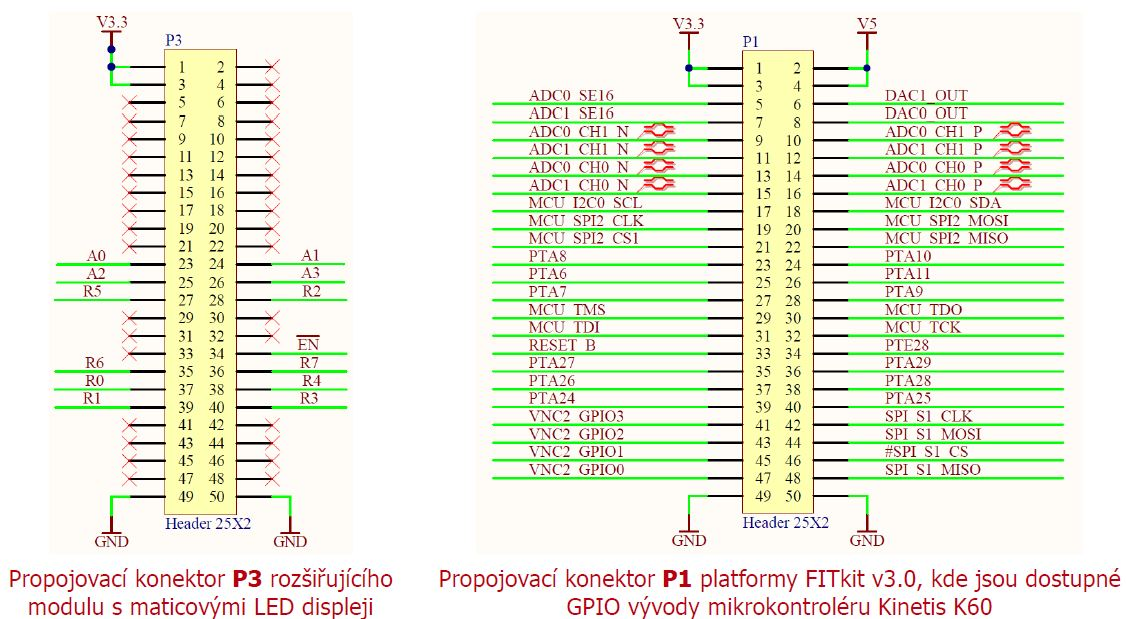
\includegraphics[width=1.0\linewidth]{zapojeni_displaye.JPG}
    \caption{Schéma zapojení konektoru P3 externího modulu na konektor P1 FITkitu 3\protect\footnotemark}
\end{figure}
    \footnotetext{ Převzato z prezentace \textbf{IMP -- projekt \uv{HAD}}, Ing. Vojtěch Mrázek, Ph.D., mrazek@fit.vutbr.cz, %
    22.10.2020, Vysoké učení technické v Brně, Fakulta informačních technologií}

GPIO vývody portu A \verb|PTA8|, \verb|PTA10|, \verb|PTA6|, \verb|PTA11| jsou napojeny
na řídící piny \verb|A0|--\verb|A3|, jejichž binární kombinace udává vybraný aktivní sloupec displaye.
Další vývody tohoto portu \verb|PTA7|, \verb|PTA9| a~\verb|PTA24|--\verb|PTA29| jsou připojeny
k řádkovým anodovým vodičům \verb|R0|--\verb|R7|, které adresují jednotlivé řádky vybraného sloupce
(log. 1 = svítí, log. 0 = nesvítí). Vývod \verb|PTE28| portu~E je napojen na pin
$\overline{\verb|EN|}$ značící negaci povolovacího signálu, tedy aby display svítil, musí zde být
přivedena logická 0.

\subsection{Ostatní použité prvky}
Kromě displaye použitého jako výstup je samozřejmě zapotřebí i~jiných prvků,
především tlačítek pro ovládání samotné hry uživatelem.
Použil jsem tlačítka \verb|BTN_SW2|--\verb|BTN_SW6|, namapované na piny portu~E
\verb|PTE10|, \verb|PTE12|, \verb|PTE27|, \verb|PTE26| a \verb|PTE11|.
Pro periodickou obsluhu displaye bylo samozřejmě zapotřebí použít nějaký časovač,
rozhodl jsem se pro Low-power timer (LPTMR).


\section{Programová realizace}
Samotný program pro MCU je napsán v jazyce C, a~nachází se v~souboru \verb|main.c|.
Tato kapitola je zaměřena na hlavní konstrukce a~mechanismy použité v~programu.
Pro řešení byl jako kostra použit zdrojový soubor z~ukázky
\verb|FITkit3-demo.zip| \footnote{ \textbf{FITkit3-demo.zip}, Ing. Michal Bidlo Ph.D., bidlom@fit.vutbr.cz, %
                        2019, Vysoké učení technické v~Brně, Fakulta informačních technologií}.
Všechny proměnné v rámci programu jsou globální, a všechny funkce (kromě \verb|int main()|) jsou typu \verb|void|.

\subsection{Inicializace portů a časovače}
Na začátku samotného programu docházi hned po inicializaci MCU funkcí \verb|MCUInit()|, kterou jsem nijak neupravoval.
Dále jsou inicializovány potřebné porty funkcí \verb|PortsInit()|. Zde jsou zapnuty hodiny
pro oba porty využívané programem, tedy port A a port E. Vybrané bity portu A řídí ovládání maticového displaye (výstup),
zatímco port E má na starost vstup z~pěti tlačítek, a navíc výstup v podobě $\overline{\verb|EN|}$ signálu displaye.
Pro oba porty jsou nastaveny odpovídající bity v registrech \verb|PTx->PCR| na hodnotu 1, jelikož jsou použity jako \verb|GPIO|.
Nakonec jsou nastaveny piny v registrech \verb|PTx->PDDR|, aby bylo zřejmé které piny jsou vstupní nebo výstupní,
a~všechny použité výstupní piny jsou v registrech \verb|PTx->PDOR| pro začátek vynulovány.
Časovač \verb|LPTMR0| je inicializován funkcí \verb|LPTMR0Init(int count)| převzaté ze zmíněného dema,
zde jsem experimentálně dospěl k~nastavení compare value na hodnotu 0, jelikož jakákoli vyšší hodnota
vedla k nedostatečné obnovovací frekvenci displaye. Také jsem zkoušel experimentovat s odlišnými časovači.

\subsection{Herní pole}
Stav herního pole je uchováván v 2D poli \verb|bool smatrix[16][8]|, kde hodnota \verb|true| na daném
indexu značí, že se zde nachází článek hada (dioda bude svítit), a velikost pole odpovídá velikosti displaye.
Pomocná funkce \verb|clearGameField(bool fill)| vyplní celé pole hodnotou \verb|fill|,
což je užitečné pro inicializaci začátku hry, ale také rozsvícení celého displaye poté, co hráč prohrál.

\subsection{Had a jeho pohyb}
Pozice hada v poli je uložena v instanci \verb|snake| struktury \verb|Snake|, která
se skládá z polí \verb|x[]| a~\verb|y[]| o~délce \verb|SNAKE_LEN| (délka hada, výchozí hodnota~8),
sloužící pro uchování horizontálních/vertikálních souřadnic jednotlivých článků hada.
Funkce \verb|setDefaultSnake()| volána vždy po startu/resetu hry nastaví hada do jeho výchozí pozice v~herním poli.
Jeho pohyb je prováděn funkcí \verb|moveSnake()|, která podle hodnoty proměnné \verb|snake_dir|
typu \verb|DIRECTION_T| udávající směr pohybu zkontroluje, zda je odpovídající buňka pole volná.
Pokud ano, celý had se posune, ale pokud se buňka nachází za hranicí pole nebo se v~ní nachází článek hada,
nastaví se hodnota proměnné \verb|bool gameOver| na \verb|true|, což způsobí konec hry a rozsvícení celého displaye.

\subsection{Obsluha přerušení od časovače}
Obsluha přerušení časovače funkcí \verb|LPTMR0_IRQHandler()| ovládá samotný display.
Nejprve jsou všechny výstupní piny pro ovládání displaye pomocí registru \verb|PTA->PDOR| vynulovány.
Proměnná \verb|int col_select| slouží k výberu aktivního sloupce a její hodnota v rozmezí 0 a 15
je inkrementována při každé obsluze přerušení. Na 4~spodní bity této proměnné jsou namapovány
bity registru \verb|PTA->PDOR| řídící výber sloupce na displayi pomocí multiplexingu. Zbývající bity řídící
zda svítí jednotlivé řádky displaye jsou poté nastaveny na základě hodnot v~herním poli
namapované na jejich pozici.
Kromě blikání displaye musí časovač obsluhovat také časování pohybu hada.
Proměnná \verb|int period_cnt| je při každém přerušení časovače inkrementována, a~když dosáhne hodnoty
\verb|PERIODS_PER_MOVE| (výchozí hodnota 384), vynuluje se a~zavolá funkci \verb|moveSnake()|.

\subsection{Smyčka obsluhy vstupů}
Při spuštění programu je kromě inicializace MCU, portů a časovače inicializováno herní pole,
nastavena výchozí poloha hada a příznak \verb|gameOver| nastaven na hodnotu \verb|false|.
S výjimkou obsluhy časovače dále celý program běží v nekonečně smyčce,
monitorující stisk jednotlivých tlačítek pomocí vstupního registru portu E \verb|GPIOE_PDIR|.
Při stisku jednoho ze 4 tlačítek řídící pohyb hada je změněn směr v proměnné \verb|snake_dir|.
Při stisku tlačítka pro resetování hry je znovu provedena inicializace herního pole, polohy hada,
a~příznaku konce hry.



\section{Výsledné řešení}
V této kapitole je výsledný program popsán spíše z~uživatelského hlediska, bez podrobných technických detailů.

\subsection{Ovládání hry}
Hra je ovládána celkově pěti tlačítky. Tlačítka \verb|SW2| až \verb|SW5| slouží ke změně směru pohybu hada,
zde je důležité podotknout, že je display postaven na výšku, tudíž jsou vlastně sloupce displaye
použité jako řádky, a řádky jako sloupce. Obsluha tlačítek je tomu přizpůsobena,
tedy had se pohybuje stejným směrem, jako je směr tlačítka při pohledu na samotné zařízení.
Tlačítko \verb|SW6| slouží k~resetu celé hry, hru lze resetovat kdykoli nehledě na její stav
(není třeba čekat až uživatel prohraje).
\begin{figure}[h!]
    \centering
    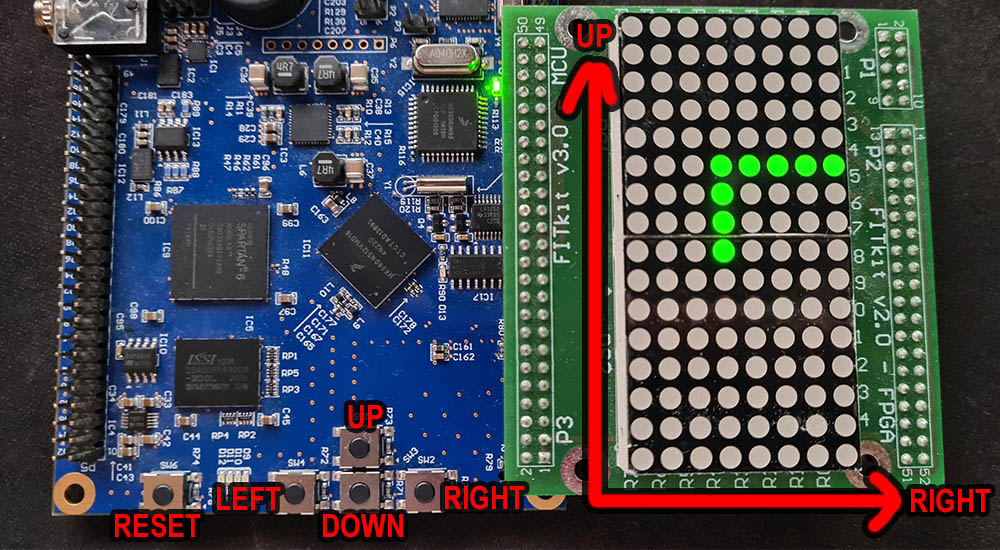
\includegraphics[width=1.0\linewidth]{conts.jpg}
    \caption{Ovládání hry pomocí tlačítek}
\end{figure}

\subsection{Funkčnost a vlastnosti řešení}
Výsledná hra umožňuje uživateli volný pohyb po herní ploše,
přičemž jsou detekovány kolize s~hranicemi a~také se samotným tělem hada,
které hru ukončí a~informují uživatele o prohře rozsvícením celého maticového displaye.
Hráč může kromě změny směru pohybu hru kdykoli resetovat, čímž navrátí hada do výchozí pozice
a~směr pohybu nastaví dopředu. Výsledná obnovovací frekvence displaye je vhodná pro dobrou
viditelnost aktivity na herní ploše, a~had provádí přibližně 3 pohyby za sekundu.
Kód hry je napsán flexibilním způsobem, změnou hodnot konstant \verb|SNAKE_LENGHT|
a~\verb|PERIODS_PER_MOVE| je snadné pozměnit velikost hada a frekvenci jeho pohybů,
pro zaručení správné funkcionality je ale vhodné se příliš nevzdalovat od výchozích hodnot.
\begin{figure}[h!]
    \centering
    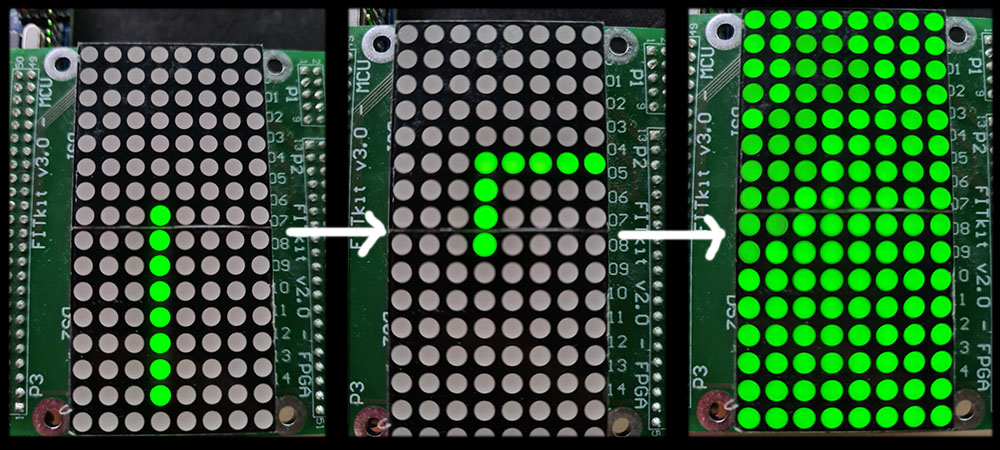
\includegraphics[width=1.0\linewidth]{prubeh.jpg}
    \caption{Ukázka průběhu hry, včetně prohry kolizí s~pravou hranicí herního pole}
\end{figure}


\section{Závěr}
Projekt jsem začal řešit už v~polovině října a~musím přiznat,
že jsem byl nejprve poměrně zmatený z~vývojového prostředí \textbf{KDS} a~také ze samotného \textbf{FITkitu 3},
který se dosti liší od jeho předchůdců. Po několika experimentech s materiály poskytnutými
v~rámci předmětu jsem se však začal v problematice lépe orientovat.
Hlavní pokrok přišel po nalezení dokumentu obsahující 
schéma zapojení maticového displaye na FITkit, viz \ref{fitkit_display_zapojeni}.
S~ovládáním maticového displaye pomocí multiplexingu jsem se již dříve setkal v~semináři VHDL (předmět \textbf{IVH}),
takže vytvořit mechanismus obsluhy displaye nebylo příliš problematické. Při řešení jsem se trochu bál,
zda není nastavení compare hodnoty časovače Low-power timer na 0 nevhodné,
s tímto nastavením se mi však podařilo dosáhnout nejlepších výsledků co se týče obnovovací frekvence displaye.
S~výsledkem jsem spokojen a~samotné programování mě celkem bavilo.
Dosti se lišilo od programování FPGA se kterým jsem se setkal v předešlých kurzech,
jedná se tedy o~kompletně novou zkušenost, což považuji za přínosné.

\begin{itemize}
    \item Původní (nekomentované) video prezentující funkčnost
    řešení: \url{https://www.youtube.com/watch?v=RqtJvzvbgGs}
    \item Obhajoba projektu formou videa: 
    \url{https://drive.google.com/file/d/1J7mCmarkUhP2P4I92j_V0exUolZ5oRXE/view?usp=sharing}
    \item Výsledek autoevaluace pomocí hodnotícího klíče: 12,6 b.
\end{itemize}




\end{document}